% !TEX TS-program = xelatex+makeindex+bibtex+shellescape
% !TEX encoding = UTF-8 Unicode



% Copyright 2024 Advaith Menon/GaTech

% Permission is hereby granted, free of charge, to any person obtaining
% a copy of this software and associated documentation files (the 
% "Software"), to deal in the Software without restriction, including
% without limitation the rights to use, copy, modify, merge, publish,
% distribute, sublicense, and/or sell copies of the Software, and to
% permit persons to whom the Software is furnished to do so, subject
% to the following conditions:

% The above copyright notice and this permission notice shall be
% included in all copies or substantial portions of the Software.

% THE SOFTWARE IS PROVIDED “AS IS”, WITHOUT WARRANTY OF ANY KIND,
% EXPRESS OR IMPLIED, INCLUDING BUT NOT LIMITED TO THE WARRANTIES
% OF MERCHANTABILITY, FITNESS FOR A PARTICULAR PURPOSE AND
% NONINFRINGEMENT. IN NO EVENT SHALL THE AUTHORS OR COPYRIGHT
% HOLDERS BE LIABLE FOR ANY CLAIM, DAMAGES OR OTHER LIABILITY,
% WHETHER IN AN ACTION OF CONTRACT, TORT OR OTHERWISE, ARISING
% FROM, OUT OF OR IN CONNECTION WITH THE SOFTWARE OR THE USE OR
% OTHER DEALINGS IN THE SOFTWARE.


% This file is a template using the "beamer" package to create slides for a 
% talk or presentation
% - Giving a talk on some subject.
% - The talk is between 15min and 45min long.
% - Style is ornate.

% MODIFIED by Jonathan Kew, 2008-07-06
% The header comments and encoding in this file were modified for inclusion
% with TeXworks.
% The content is otherwise unchanged from the original distributed with the
% beamer package.

\documentclass{beamer}


% Copyright 2004 by Till Tantau <tantau@users.sourceforge.net>.
%
% In principle, this file can be redistributed and/or modified under
% the terms of the GNU General Public License, version 2.
%
% However, this file is supposed to be a template to be modified
% for your own needs. For this reason, if you use this file as a
% template and not specifically distribute it as part of a another
% package/program, I grant the extra permission to freely copy and
% modify this file as you see fit and even to delete this copyright
% notice. 


\mode<presentation>
{
  % \usetheme{Warsaw}
  \usetheme{Singapore}
  % or ...

  % \setbeamercovered{transparent}
  % or whatever (possibly just delete it)
}
\usefonttheme[onlymath]{serif}
\setbeamertemplate{caption}[numbered]
\setbeamerfont{footnote}{size=\tiny}


\usepackage[english]{babel}
%\usepackage{enumitem}
\usepackage{multicol}
\usepackage{environ}
\usepackage{pgffor}
\usepackage{minted}
\usepackage{pgfplots}
\pgfplotsset{height=0.8\textheight,compat=1.9}

% or whatever

\usepackage[utf8]{inputenc}
% or whatever

\usepackage{times}
\usepackage[T1]{fontenc}
% Or whatever. Note that the encoding and the font should match. If T1
% does not look nice, try deleting the line with the fontenc.

% tikz stuff
\usetikzlibrary{decorations.pathmorphing,patterns}

\newcounter{boxCounter}
\newsavebox{\boxA}
\newsavebox{\boxB}
\newsavebox{\boxC}
\newsavebox{\boxD}


\newlength{\availafter}

\NewEnviron{autotext}[1][0.5cm]
{\setcounter{boxCounter}{0}\foreach \mysize in {\normalsize,\small,\footnotesize,\scriptsize}{\stepcounter{boxCounter}\expandafter\savebox\csname box\Alph{boxCounter}\endcsname{\vbox{\mysize\BODY}}\setlength{\availafter}{\dimexpr\textheight-\expandafter\ht\csname box\Alph{boxCounter}\endcsname-\pagetotal\relax}\ifdim\availafter>#1\expandafter\usebox\csname box\Alph{boxCounter}\endcsname\breakforeach\fi}}



\title[PHYS-2211-Lab04] % (optional, use only with long paper titles)
{Physics 2211 - Lab 4}

\subtitle
{Oscillations} % (optional)

\author[Menon, Advaith] % (optional, use only with lots of authors)
{Advaith~Menon\inst{1}}
% - Use the \inst{?} command only if the authors have different
%   affiliation.

\institute%[Universities of Somewhere and Elsewhere] % (optional, but mostly needed)
{
  \inst{1}%
  Computer Engineering\\
  Georgia Institute of Technology
  }
% - Use the \inst command only if there are several affiliations.
% - Keep it simple, no one is interested in your street address.

\date%[Short Occasion] % (optional)
{March 13\textsuperscript{th}, 2024}

\subject{Physics Lab}
% This is only inserted into the PDF information catalog. Can be left
% out. 



% If you have a file called "university-logo-filename.xxx", where xxx
% is a graphic format that can be processed by latex or pdflatex,
% resp., then you can add a logo as follows:

\pgfdeclareimage[height=0.5cm]{university-logo}{img/GeorgiaTechLogo}
\logo{\pgfuseimage{university-logo}}



% Delete this, if you do not want the table of contents to pop up at
% the beginning of each subsection:
%\AtBeginSubsection[]
\AtBeginSection[]
{
  \begin{frame}<beamer>{Outline}
    \tableofcontents[currentsection]  %,currentsubsection
  \end{frame}
}


% If you wish to uncover everything in a step-wise fashion, uncomment
% the following command: 

%\beamerdefaultoverlayspecification{<+->}


\begin{document}

\begin{frame}
  \titlepage
\end{frame}

\begin{frame}{Outline}
  \tableofcontents
  % You might wish to add the option [pausesections]
\end{frame}


% Since this a solution template for a generic talk, very little can
% be said about how it should be structured. However, the talk length
% of between 15min and 45min and the theme suggest that you stick to
% the following rules:  

% - Exactly two or three sections (other than the summary).
% - At *most* three subsections per section.
% - Talk about 30s to 2min per frame. So there should be between about
%   15 and 30 frames, all told.

%%%%% BEGIN SLIDES %%%%%

% !TEX TS-program = xelatex+makeindex+bibtex+shellescape
% !TEX encoding = UTF-8 Unicode

% Copyright 2024 Advaith Menon/GaTech

% Permission is hereby granted, free of charge, to any person obtaining
% a copy of this software and associated documentation files (the 
% "Software"), to deal in the Software without restriction, including
% without limitation the rights to use, copy, modify, merge, publish,
% distribute, sublicense, and/or sell copies of the Software, and to
% permit persons to whom the Software is furnished to do so, subject
% to the following conditions:

% The above copyright notice and this permission notice shall be
% included in all copies or substantial portions of the Software.

% THE SOFTWARE IS PROVIDED “AS IS”, WITHOUT WARRANTY OF ANY KIND,
% EXPRESS OR IMPLIED, INCLUDING BUT NOT LIMITED TO THE WARRANTIES
% OF MERCHANTABILITY, FITNESS FOR A PARTICULAR PURPOSE AND
% NONINFRINGEMENT. IN NO EVENT SHALL THE AUTHORS OR COPYRIGHT
% HOLDERS BE LIABLE FOR ANY CLAIM, DAMAGES OR OTHER LIABILITY,
% WHETHER IN AN ACTION OF CONTRACT, TORT OR OTHERWISE, ARISING
% FROM, OUT OF OR IN CONNECTION WITH THE SOFTWARE OR THE USE OR
% OTHER DEALINGS IN THE SOFTWARE.

% Intro slides

\section{Introduction}
% !TEX TS-program = xelatex+makeindex+bibtex+shellescape
% !TEX encoding = UTF-8 Unicode

% Copyright 2024 Advaith Menon/GaTech

% Permission is hereby granted, free of charge, to any person obtaining
% a copy of this software and associated documentation files (the 
% "Software"), to deal in the Software without restriction, including
% without limitation the rights to use, copy, modify, merge, publish,
% distribute, sublicense, and/or sell copies of the Software, and to
% permit persons to whom the Software is furnished to do so, subject
% to the following conditions:

% The above copyright notice and this permission notice shall be
% included in all copies or substantial portions of the Software.

% THE SOFTWARE IS PROVIDED “AS IS”, WITHOUT WARRANTY OF ANY KIND,
% EXPRESS OR IMPLIED, INCLUDING BUT NOT LIMITED TO THE WARRANTIES
% OF MERCHANTABILITY, FITNESS FOR A PARTICULAR PURPOSE AND
% NONINFRINGEMENT. IN NO EVENT SHALL THE AUTHORS OR COPYRIGHT
% HOLDERS BE LIABLE FOR ANY CLAIM, DAMAGES OR OTHER LIABILITY,
% WHETHER IN AN ACTION OF CONTRACT, TORT OR OTHERWISE, ARISING
% FROM, OUT OF OR IN CONNECTION WITH THE SOFTWARE OR THE USE OR
% OTHER DEALINGS IN THE SOFTWARE.

% Aim slide

\subsection[Aim]{Aim of the experiment}
\begin{frame}{Aim}{Purpose of this lab assignment}
    \begin{itemize}
    \item Analyze the motion of a mass oscillating under the effect of spring force and gravity
    \item Verify the energy principle for this system.
    \end{itemize}
\end{frame}
% !TEX TS-program = xelatex+makeindex+bibtex+shellescape
% !TEX encoding = UTF-8 Unicode

% Copyright 2024 Advaith Menon/GaTech

% Permission is hereby granted, free of charge, to any person obtaining
% a copy of this software and associated documentation files (the 
% "Software"), to deal in the Software without restriction, including
% without limitation the rights to use, copy, modify, merge, publish,
% distribute, sublicense, and/or sell copies of the Software, and to
% permit persons to whom the Software is furnished to do so, subject
% to the following conditions:

% The above copyright notice and this permission notice shall be
% included in all copies or substantial portions of the Software.

% THE SOFTWARE IS PROVIDED “AS IS”, WITHOUT WARRANTY OF ANY KIND,
% EXPRESS OR IMPLIED, INCLUDING BUT NOT LIMITED TO THE WARRANTIES
% OF MERCHANTABILITY, FITNESS FOR A PARTICULAR PURPOSE AND
% NONINFRINGEMENT. IN NO EVENT SHALL THE AUTHORS OR COPYRIGHT
% HOLDERS BE LIABLE FOR ANY CLAIM, DAMAGES OR OTHER LIABILITY,
% WHETHER IN AN ACTION OF CONTRACT, TORT OR OTHERWISE, ARISING
% FROM, OUT OF OR IN CONNECTION WITH THE SOFTWARE OR THE USE OR
% OTHER DEALINGS IN THE SOFTWARE.

% Intro slides

\section{Prerequisites}
% !TEX TS-program = xelatex+makeindex+bibtex+shellescape
% !TEX encoding = UTF-8 Unicode

% Copyright 2024 Advaith Menon/GaTech

% Permission is hereby granted, free of charge, to any person obtaining
% a copy of this software and associated documentation files (the 
% "Software"), to deal in the Software without restriction, including
% without limitation the rights to use, copy, modify, merge, publish,
% distribute, sublicense, and/or sell copies of the Software, and to
% permit persons to whom the Software is furnished to do so, subject
% to the following conditions:

% The above copyright notice and this permission notice shall be
% included in all copies or substantial portions of the Software.

% THE SOFTWARE IS PROVIDED “AS IS”, WITHOUT WARRANTY OF ANY KIND,
% EXPRESS OR IMPLIED, INCLUDING BUT NOT LIMITED TO THE WARRANTIES
% OF MERCHANTABILITY, FITNESS FOR A PARTICULAR PURPOSE AND
% NONINFRINGEMENT. IN NO EVENT SHALL THE AUTHORS OR COPYRIGHT
% HOLDERS BE LIABLE FOR ANY CLAIM, DAMAGES OR OTHER LIABILITY,
% WHETHER IN AN ACTION OF CONTRACT, TORT OR OTHERWISE, ARISING
% FROM, OUT OF OR IN CONNECTION WITH THE SOFTWARE OR THE USE OR
% OTHER DEALINGS IN THE SOFTWARE.

% Newton's Second law slides

\subsection{Newton's Second Law}
\begin{frame}{Newton's Second Law}{Quantitative analysis of motion}
	``The net force acting on a body is defined as the change in its 
	momentum per unit time.''
	\begin{equation}
	\vec{F}_{net} = \frac{\mathrm{d}\vec{p}}{\mathrm{d}t}
	\end{equation}
	In most daily life scenarios, mass doesn't change with respect to
	time, hence this equation is better known as:
	\[\vec{F}_{net} = m\cdot\vec{a}\]
	where,
	\begin{itemize}
	\item \(\vec{F}_{net} = \) Net force acting on a body
	\item \(m = \) Mass of the body
	\item \(\vec{a} = \frac{\mathrm{d}\vec{v}}{\mathrm{d}t} 
		= \frac{\mathrm{d}^2\vec{r}}{\mathrm{d}t^2} = \) 
		Net acceleration on body	
	\item \(\Delta\vec{p} = m\times\Delta\vec{v} = \)
		Change in momentum
	\end{itemize}
\end{frame}

\begin{frame}{Corollary: The Momentum Principle}{Rearranging the equation}
	\begin{equation}
	\Delta \vec{p} = \vec{F}_{net} \times {\Delta t}
	\end{equation}
	where,
	\begin{itemize}
	\item \(\vec{F}_{net} = \) Net force acting on a body	
	\item \(\Delta\vec{p} = \)
		Change in momentum
	\end{itemize}
\end{frame}
% !TEX TS-program = xelatex+makeindex+bibtex+shellescape
% !TEX encoding = UTF-8 Unicode

% Copyright 2024 Advaith Menon/GaTech

% Permission is hereby granted, free of charge, to any person obtaining
% a copy of this software and associated documentation files (the 
% "Software"), to deal in the Software without restriction, including
% without limitation the rights to use, copy, modify, merge, publish,
% distribute, sublicense, and/or sell copies of the Software, and to
% permit persons to whom the Software is furnished to do so, subject
% to the following conditions:

% The above copyright notice and this permission notice shall be
% included in all copies or substantial portions of the Software.

% THE SOFTWARE IS PROVIDED “AS IS”, WITHOUT WARRANTY OF ANY KIND,
% EXPRESS OR IMPLIED, INCLUDING BUT NOT LIMITED TO THE WARRANTIES
% OF MERCHANTABILITY, FITNESS FOR A PARTICULAR PURPOSE AND
% NONINFRINGEMENT. IN NO EVENT SHALL THE AUTHORS OR COPYRIGHT
% HOLDERS BE LIABLE FOR ANY CLAIM, DAMAGES OR OTHER LIABILITY,
% WHETHER IN AN ACTION OF CONTRACT, TORT OR OTHERWISE, ARISING
% FROM, OUT OF OR IN CONNECTION WITH THE SOFTWARE OR THE USE OR
% OTHER DEALINGS IN THE SOFTWARE.

% Newton's Second law slides

\subsection{Hooke's Law}
\begin{frame}{Hooke's Law}{Measuring spring forces}
	``The magnitude of the force exerted by a stretched spring is directly proportional to its change in length.''
	\begin{equation}
	\vec{F}_{s} = - k \left(L - L_0\right) \hat{L}
	\end{equation}
	where,
	\begin{itemize}
	\item \(\vec{F}_s = \) The vector force exerted by the spring.
    \item \(L = \) The current length of the spring (scalar).
    \item \(\hat{L} = \) The unit vector pointing from the fixed end of the spring to the free end.
    \item \(L_0 = \) The natural length of the spring.
	\end{itemize}
\end{frame}
% !TEX TS-program = xelatex+makeindex+bibtex+shellescape
% !TEX encoding = UTF-8 Unicode

% Copyright 2024 Advaith Menon/GaTech

% Permission is hereby granted, free of charge, to any person obtaining
% a copy of this software and associated documentation files (the 
% "Software"), to deal in the Software without restriction, including
% without limitation the rights to use, copy, modify, merge, publish,
% distribute, sublicense, and/or sell copies of the Software, and to
% permit persons to whom the Software is furnished to do so, subject
% to the following conditions:

% The above copyright notice and this permission notice shall be
% included in all copies or substantial portions of the Software.

% THE SOFTWARE IS PROVIDED “AS IS”, WITHOUT WARRANTY OF ANY KIND,
% EXPRESS OR IMPLIED, INCLUDING BUT NOT LIMITED TO THE WARRANTIES
% OF MERCHANTABILITY, FITNESS FOR A PARTICULAR PURPOSE AND
% NONINFRINGEMENT. IN NO EVENT SHALL THE AUTHORS OR COPYRIGHT
% HOLDERS BE LIABLE FOR ANY CLAIM, DAMAGES OR OTHER LIABILITY,
% WHETHER IN AN ACTION OF CONTRACT, TORT OR OTHERWISE, ARISING
% FROM, OUT OF OR IN CONNECTION WITH THE SOFTWARE OR THE USE OR
% OTHER DEALINGS IN THE SOFTWARE.

% Newton's Second law slides

\subsection{Energy Principle}
\begin{frame}{Energy Principle}
	``The change in energy of a system is equivalent to the external work done on it.''
	\begin{equation}
	\Delta E = W_{ext}
	\end{equation}
	where,
	\begin{itemize}
	\item \(\Delta E = \) Change in energy of the system.
    \item \(W_{ext} = \) The external work done by the surroundings.
	\end{itemize}
\end{frame}
% !TEX TS-program = xelatex+makeindex+bibtex+shellescape
% !TEX encoding = UTF-8 Unicode

% Copyright 2024 Advaith Menon/GaTech

% Permission is hereby granted, free of charge, to any person obtaining
% a copy of this software and associated documentation files (the 
% "Software"), to deal in the Software without restriction, including
% without limitation the rights to use, copy, modify, merge, publish,
% distribute, sublicense, and/or sell copies of the Software, and to
% permit persons to whom the Software is furnished to do so, subject
% to the following conditions:

% The above copyright notice and this permission notice shall be
% included in all copies or substantial portions of the Software.

% THE SOFTWARE IS PROVIDED “AS IS”, WITHOUT WARRANTY OF ANY KIND,
% EXPRESS OR IMPLIED, INCLUDING BUT NOT LIMITED TO THE WARRANTIES
% OF MERCHANTABILITY, FITNESS FOR A PARTICULAR PURPOSE AND
% NONINFRINGEMENT. IN NO EVENT SHALL THE AUTHORS OR COPYRIGHT
% HOLDERS BE LIABLE FOR ANY CLAIM, DAMAGES OR OTHER LIABILITY,
% WHETHER IN AN ACTION OF CONTRACT, TORT OR OTHERWISE, ARISING
% FROM, OUT OF OR IN CONNECTION WITH THE SOFTWARE OR THE USE OR
% OTHER DEALINGS IN THE SOFTWARE.

% Initial conditions, system and surroundings, FBD

\subsection{Initial Conditions}
\begin{frame}{Initial Conditions}
	\begin{itemize}
	\item Initial position, \(\vec{r}_i = 0\hat{i} + 1.12\times 10^{-2} \hat{j} + 0\hat{k}\ \mathrm{m} \)
	\item Mass of the ball, \(m_{ball} = 4.6\ \mathrm{g} = 4.6 \times 10^{-3}\ \mathrm{kg}\)
	\end{itemize}
\end{frame}

\begin{frame}{System and Surroundings}
	\begin{itemize}
	\item \textbf{System:} Paper ball (hereafter referred to as `object')
	\item \textbf{Surroundings:} Everything else (table, air, etc.)
	\end{itemize}
\end{frame}

\begin{frame}{Free-Body Diagram}
    \begin{center}
	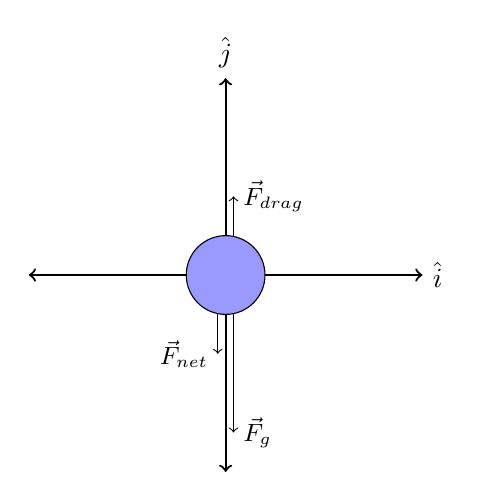
\begin{tikzpicture}[scale=0.5]
    % axes
    % \draw[step=1cm,gray,very thin] (-5, -5) grid (5, 5);
    \draw[thick,->] (0, 0) -- (0, 5) node[anchor=south] {\(\hat{j}\)};
    \draw[thick,->] (0, 0) -- (5, 0) node[anchor=west] {\(\hat{i}\)};
    \draw[thick,->] (0, 0) -- (0, -5);
    \draw[thick,->] (0, 0) -- (-5, 0);
    % forces
    \draw[->] (0.2, 0) -- (0.2, -4) node[font=\small, anchor=west] {\(\vec{F}_g\)};
    \draw[->] (0.2, 0) -- (0.2, 2) node[font=\small, anchor=west] {\(\vec{F}_{drag}\)};
    \draw[->] (-0.2, 0) -- (-0.2, -2) node[font=\small, anchor=east] {\(\vec{F}_{net}\)};
    % ball
    \fill[blue!40!white, draw=black] (0, 0) circle (1cm);
    \end{tikzpicture}
    \end{center}
\end{frame}
% !TEX TS-program = xelatex+makeindex+bibtex+shellescape
% !TEX encoding = UTF-8 Unicode

% Copyright 2024 Advaith Menon/GaTech

% Permission is hereby granted, free of charge, to any person obtaining
% a copy of this software and associated documentation files (the 
% "Software"), to deal in the Software without restriction, including
% without limitation the rights to use, copy, modify, merge, publish,
% distribute, sublicense, and/or sell copies of the Software, and to
% permit persons to whom the Software is furnished to do so, subject
% to the following conditions:

% The above copyright notice and this permission notice shall be
% included in all copies or substantial portions of the Software.

% THE SOFTWARE IS PROVIDED “AS IS”, WITHOUT WARRANTY OF ANY KIND,
% EXPRESS OR IMPLIED, INCLUDING BUT NOT LIMITED TO THE WARRANTIES
% OF MERCHANTABILITY, FITNESS FOR A PARTICULAR PURPOSE AND
% NONINFRINGEMENT. IN NO EVENT SHALL THE AUTHORS OR COPYRIGHT
% HOLDERS BE LIABLE FOR ANY CLAIM, DAMAGES OR OTHER LIABILITY,
% WHETHER IN AN ACTION OF CONTRACT, TORT OR OTHERWISE, ARISING
% FROM, OUT OF OR IN CONNECTION WITH THE SOFTWARE OR THE USE OR
% OTHER DEALINGS IN THE SOFTWARE.

% Experiment slides

\section{Experiment}
% !TEX TS-program = xelatex+makeindex+bibtex+shellescape
% !TEX encoding = UTF-8 Unicode

% Copyright 2024 Advaith Menon/GaTech

% Permission is hereby granted, free of charge, to any person obtaining
% a copy of this software and associated documentation files (the 
% "Software"), to deal in the Software without restriction, including
% without limitation the rights to use, copy, modify, merge, publish,
% distribute, sublicense, and/or sell copies of the Software, and to
% permit persons to whom the Software is furnished to do so, subject
% to the following conditions:

% The above copyright notice and this permission notice shall be
% included in all copies or substantial portions of the Software.

% THE SOFTWARE IS PROVIDED “AS IS”, WITHOUT WARRANTY OF ANY KIND,
% EXPRESS OR IMPLIED, INCLUDING BUT NOT LIMITED TO THE WARRANTIES
% OF MERCHANTABILITY, FITNESS FOR A PARTICULAR PURPOSE AND
% NONINFRINGEMENT. IN NO EVENT SHALL THE AUTHORS OR COPYRIGHT
% HOLDERS BE LIABLE FOR ANY CLAIM, DAMAGES OR OTHER LIABILITY,
% WHETHER IN AN ACTION OF CONTRACT, TORT OR OTHERWISE, ARISING
% FROM, OUT OF OR IN CONNECTION WITH THE SOFTWARE OR THE USE OR
% OTHER DEALINGS IN THE SOFTWARE.

% Observations - Tracker
\subsection{Observation}
\begin{frame}{Analysis of Video}{Getting displacement, velocity, acceleration at discrete time intervals using Tracker}
\begin{figure}
\centering
    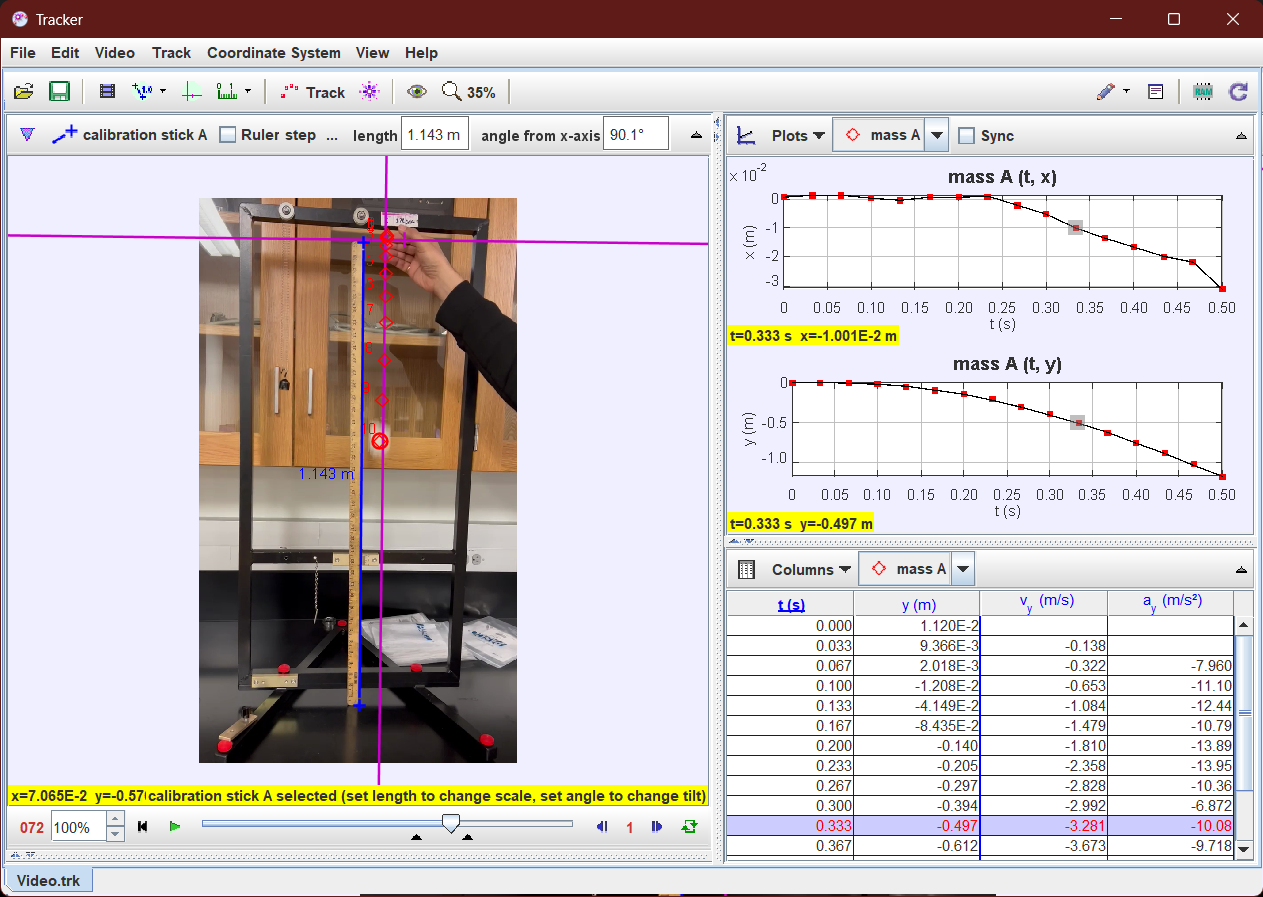
\includegraphics[height=0.7\textheight]{img/trackerSS}
    \caption{Using Tracker\textsuperscript{\textregistered} to analyze the motion of the object.}
    \label{fig:trackerSS}
\end{figure}
\end{frame}

\begin{frame}{Calculating Acceleration}
\begin{columns}
\begin{column}{0.5\textwidth}
   \begin{center}
   \begin{tabular}{|r|r|}
    \hline
    \textbf{Time} \(t\) (s) & \textbf{Y-Position} \(r_y\) (m) \\
    \hline
    0.00E+00 & 1.12E-02 \\
    \hline
    3.33E-02 & 9.37E-03  \\
    \hline
    6.67E-02 & 2.02E-03  \\
    \hline
    1.00E-01 & -1.21E-02 \\
    \hline
    1.33E-01 & -4.15E-02 \\
    \hline
    1.67E-01 & -8.43E-02 \\
	\hline
	\multicolumn{2}{|c|}{\vdots\ \ \ \ \ \ \ \ \ \ \ \ \vdots} \\
	\hline
   \end{tabular}
   \end{center}
\end{column}
\begin{column}{0.5\textwidth}
	\begin{itemize}
		\item \[\vec{v}_{avg,2} = \frac{\vec{r}_3-\vec{r}_1}
				{t_3-t_1}\]
		\item Unlike the last lab, slightly larger time intervals have been
        used to ensure more accuracy.
	\end{itemize}
\end{column}
\end{columns}
\end{frame}

\begin{frame}{Calculating Acceleration}
\begin{columns}
\begin{column}{0.4\textwidth}
    \begin{autotext}
    \begin{itemize}
    \item Repeating this step multiple times, we can get the average
        velocity for each interval
    \item Next step - calculate the acceleration
        \[\vec{a}_{avg,3} = \frac{\vec{v}_4-\vec{v}_2}
				{t_4-t_2}\]
    \end{itemize}
    \end{autotext}
\end{column}
\begin{column}{0.6\textwidth}
	\begin{center}
    \small
    \begin{tabular}{|c|c|c|}
    \hline
    \(t\) (s) & \(r_y\) (m) & \(v_y\) (m) \\
    \hline
    0.00E+00 & 1.12E-02 &  \\
    \hline
    3.33E-02 & 9.37E-03 & -1.38E-01 \\
    \hline
    6.67E-02 & 2.02E-03 & -3.22E-01 \\
    \hline
    1.00E-01 & -1.21E-02 & -6.53E-01 \\
    \hline
    1.33E-01 & -4.15E-02 & -1.08E+00 \\
    \hline
    1.67E-01 & -8.43E-02 & -1.48E+00 \\
    \hline
	\multicolumn{3}{|c|}{\vdots\ \ \ \ \ \ \ \ \ \ \ \ \vdots} \\
	\hline
   \end{tabular}
   \end{center}
\end{column}
\end{columns}
\end{frame}

\begin{frame}{Calculating Acceleration}{Some things to keep in mind}
    \begin{itemize}
	\item Repeating this step multiple times, we can get the average
		acceleration for each interval
	\item Ideally, the average acceleration for each interval should be 
		constant, but due to various factors such as air resistance
		, friction on the surface, etc, the acceleration is not constant. 
	\item Hence, we average the accelerations of these small steps to get an 
	accurate reading.
	\end{itemize}
\end{frame}
% !TEX TS-program = xelatex+makeindex+bibtex+shellescape
% !TEX encoding = UTF-8 Unicode

% Copyright 2024 Advaith Menon/GaTech

% Permission is hereby granted, free of charge, to any person obtaining
% a copy of this software and associated documentation files (the 
% "Software"), to deal in the Software without restriction, including
% without limitation the rights to use, copy, modify, merge, publish,
% distribute, sublicense, and/or sell copies of the Software, and to
% permit persons to whom the Software is furnished to do so, subject
% to the following conditions:

% The above copyright notice and this permission notice shall be
% included in all copies or substantial portions of the Software.

% THE SOFTWARE IS PROVIDED “AS IS”, WITHOUT WARRANTY OF ANY KIND,
% EXPRESS OR IMPLIED, INCLUDING BUT NOT LIMITED TO THE WARRANTIES
% OF MERCHANTABILITY, FITNESS FOR A PARTICULAR PURPOSE AND
% NONINFRINGEMENT. IN NO EVENT SHALL THE AUTHORS OR COPYRIGHT
% HOLDERS BE LIABLE FOR ANY CLAIM, DAMAGES OR OTHER LIABILITY,
% WHETHER IN AN ACTION OF CONTRACT, TORT OR OTHERWISE, ARISING
% FROM, OUT OF OR IN CONNECTION WITH THE SOFTWARE OR THE USE OR
% OTHER DEALINGS IN THE SOFTWARE.

% Observations - Tracker
\subsection{Model (without drag)}
\begin{frame}{Model (without drag)}{Data needed for simulation}
\begin{itemize}
    \item Net acceleration on object, \texttt{a\_net} \( = -g\hat{j}\)
     ms\textsuperscript{-2} \( = -9.8\hat{j}\) ms\textsuperscript{-2}
    \item Vertical displacement, \texttt{delta\_h} \( = -1.17\hat{j}\) m
    \item Initial position \( = 1.12\times 10^{-2} \hat{j} \) m
    \item Mass of the ball, \(m_{ball} = 4.6\ \mathrm{g} = 4.6 \times 10^{-3}
    \ \mathrm{kg}\)
\end{itemize}
\end{frame}

\begin{frame}[fragile]{Model (without drag)}{Simulation code}
\begin{multicols}{2}
\begin{minted}[breaklines,fontsize=\tiny]{python}
# CONSTANTS
ACC_G = 9.8 # ms-2

ball = sphere(color=color.blue, radius=0.22) # sphere ball = new sphere(color.BLUE, 0.22);
trail = curve(color=color.green, radius=0.02)
origin = sphere(pos=vector(0,0,0), color=color.yellow, radius=0.04)
plot = graph(title="Position vs Time", xtitle="Time (s)", ytitle="Position (m)")
poscurve = gcurve(color=color.green, width=4)
plot = graph(title="Velocity vs Time", xtitle="Time (s)", ytitle="Velocity (m/s)")
velcurve = gcurve(color=color.green, width=4)
plot = graph(title="Acceleration vs Time", xtitle="Time (s)", ytitle="Velocity (m/s2)")
acccurve = gcurve(color=color.green, width=4)

# SYSTEM PROPERTIES & INITIAL CONDITIONS
ball.m = 4.6e-3 #kg
ball.pos = vector(0,1.12e-2,0) # m
ball.vel = vector(0,0,0) # 
ball.acc = vector(0, -ACC_G, 0) #ms-2

# Time
t = 0           # where the clock starts
deltat = 0.001   # size of each timestep

while ball.pos.y >= -1.157057:
    rate(1000)
    
    # Apply the Momentum Principle (Newton's 2nd Law)
    ball.vel = ball.vel + ball.acc*deltat
    ball.pos = ball.pos + ball.vel*deltat
    
    t = t + deltat
    trail.append(pos=ball.pos)

    poscurve.plot(t,ball.pos.y)
    velcurve.plot(t,ball.vel.y)
    acccurve.plot(t,ball.acc.y);
    print(t,ball.pos.x)

print("All done!")
\end{minted}
\end{multicols}
\end{frame}
% !TEX TS-program = xelatex+makeindex+bibtex+shellescape
% !TEX encoding = UTF-8 Unicode

% Copyright 2024 Advaith Menon/GaTech

% Permission is hereby granted, free of charge, to any person obtaining
% a copy of this software and associated documentation files (the 
% "Software"), to deal in the Software without restriction, including
% without limitation the rights to use, copy, modify, merge, publish,
% distribute, sublicense, and/or sell copies of the Software, and to
% permit persons to whom the Software is furnished to do so, subject
% to the following conditions:

% The above copyright notice and this permission notice shall be
% included in all copies or substantial portions of the Software.

% THE SOFTWARE IS PROVIDED “AS IS”, WITHOUT WARRANTY OF ANY KIND,
% EXPRESS OR IMPLIED, INCLUDING BUT NOT LIMITED TO THE WARRANTIES
% OF MERCHANTABILITY, FITNESS FOR A PARTICULAR PURPOSE AND
% NONINFRINGEMENT. IN NO EVENT SHALL THE AUTHORS OR COPYRIGHT
% HOLDERS BE LIABLE FOR ANY CLAIM, DAMAGES OR OTHER LIABILITY,
% WHETHER IN AN ACTION OF CONTRACT, TORT OR OTHERWISE, ARISING
% FROM, OUT OF OR IN CONNECTION WITH THE SOFTWARE OR THE USE OR
% OTHER DEALINGS IN THE SOFTWARE.

% Observations - Tracker
\subsection{Model (with drag)}
\begin{frame}{Model (with drag)}{Data needed for simulation}
\begin{itemize}
    \item Net acceleration on object, \texttt{a\_net} \( = -g\hat{j}\)
     ms\textsuperscript{-2} \( = -9.8\hat{j}\) ms\textsuperscript{-2}
    \item Vertical displacement, \texttt{delta\_h} \( = -1.17\hat{j}\) m
    \item Initial position \( = 1.12\times 10^{-2} \hat{j} \) m
    \item Mass of the ball, \(m_{ball} = 4.6\ \mathrm{g} = 4.6 \times 10^{-3}
    \ \mathrm{kg}\)
    \item \textbf{NOTE}: The data stays the same, the only thing to keep in 
    mind is that we have to account for drag force too!
    \item \texttt{drag\_force} = \(b|v|^2 \hat{j}\)
\end{itemize}
\end{frame}

\begin{frame}[fragile]{Model (with drag)}{Simulation code}
\begin{multicols}{2}
\begin{minted}[breaklines,fontsize=\tiny]{python}
# CONSTANTS
ACC_G = 9.8 # ms-2
B = .001 # guessed by trial-and-error

ball = sphere(color=color.blue, radius=0.22) # sphere ball = new sphere(color.BLUE, 0.22);
trail = curve(color=color.green, radius=0.02)
origin = sphere(pos=vector(0,0,0), color=color.yellow, radius=0.04)
plot = graph(title="Position vs Time", xtitle="Time (s)", ytitle="Position (m)")
poscurve = gcurve(color=color.green, width=4)
plot = graph(title="Velocity vs Time", xtitle="Time (s)", ytitle="Velocity (m/s)")
velcurve = gcurve(color=color.green, width=4)
plot = graph(title="Acceleration vs Time", xtitle="Time (s)", ytitle="Velocity (m/s2)")
acccurve = gcurve(color=color.green, width=4)

# SYSTEM PROPERTIES & INITIAL CONDITIONS
ball.m = 4.6e-3 #kg
ball.pos = vector(0,1.12e-2,0) # m
ball.vel = vector(0,0,0) # 
ball.acc = vector(0, -ACC_G, 0) #ms-2

# Time
t = 0           # where the clock starts
deltat = 0.001   # size of each timestep

while ball.pos.y >= -1.157057:
    rate(1000)

    # Apply the Momentum Principle (Newton's 2nd Law)
    acc = (ball.acc + (B*ball.vel.y**2/ball.m)*vector(0, 1, 0))
    ball.vel = ball.vel + acc*deltat
    ball.pos = ball.pos + ball.vel*deltat
    
    t = t + deltat
    trail.append(pos=ball.pos)

    poscurve.plot(t,ball.pos.y)
    velcurve.plot(t,ball.vel.y)
    acccurve.plot(t,acc.y);
    print(t,ball.pos.x)

print("All done!")
\end{minted}
\end{multicols}
\end{frame}
\subsection{Comparison of Results}
\begin{frame}[fragile]{Comparison of Results}{Predicted vs. real}
\begin{center}
\begin{tikzpicture}
\begin{axis}[
    title={Position vs. time graph of dropped object},
    xlabel={Time [s]},
    ylabel={Position [m]},
    xmin=0, xmax=0.5,
    ymin=-1.2, ymax=0.2,
    xtick={0, 0.1, 0.2, 0.3, 0.4, 0.5},
    ytick={0.2, 0, -0.2, -0.4, -0.6, -0.8, -1, -1.2},
    legend pos=north east,
    ymajorgrids=true,
    grid style=dashed,
]

\addplot[
    color=red,
    mark=o,
    ]
    coordinates {
    (0.000000, 0.011196)
    (0.033333, 0.009366)
    (0.066667, 0.002018)
    (0.100000, -0.012082)
    (0.133333, -0.041490)
    (0.166667, -0.084349)
    (0.200000, -0.140082)
    (0.233333, -0.205001)
    (0.266667, -0.297275)
    (0.300000, -0.393568)
    (0.333333, -0.496760)
    (0.366667, -0.612309)
    (0.400000, -0.741607)
    (0.433333, -0.875717)
    (0.466667, -1.015310)
    (0.500000, -1.157057)};
\addlegendentry{\tiny Actual positions}
    
\addplot[
    color=brown,
    mark=,
    ]
    coordinates {
    (0.001, 0.011190199999999999)
    (0.002, 0.0111706)
    (0.003, 0.011141199999999999)
    (0.004, 0.011101999999999999)
    (0.005, 0.011052999999999999)
    (0.006, 0.010994199999999999)
    (0.007, 0.010925599999999999)
    (0.008, 0.0108472)
    (0.009000000000000001, 0.010759)
    (0.010000000000000002, 0.010660999999999999)
    (0.011000000000000003, 0.010553199999999999)
    (0.012000000000000004, 0.010435599999999998)
    (0.013000000000000005, 0.010308199999999998)
    (0.014000000000000005, 0.010170999999999998)
    (0.015000000000000006, 0.010023999999999998)
    (0.016000000000000007, 0.009867199999999998)
    (0.017000000000000008, 0.009700599999999998)
    (0.01800000000000001, 0.009524199999999998)
    (0.01900000000000001, 0.009337999999999999)
    (0.02000000000000001, 0.009141999999999999)
    (0.02100000000000001, 0.008936199999999998)
    (0.022000000000000013, 0.008720599999999998)
    (0.023000000000000013, 0.008495199999999998)
    (0.024000000000000014, 0.008259999999999998)
    (0.025000000000000015, 0.008014999999999998)
    (0.026000000000000016, 0.0077601999999999975)
    (0.027000000000000017, 0.007495599999999997)
    (0.028000000000000018, 0.007221199999999997)
    (0.02900000000000002, 0.006936999999999997)
    (0.03000000000000002, 0.006642999999999997)
    (0.03100000000000002, 0.006339199999999997)
    (0.03200000000000002, 0.006025599999999997)
    (0.03300000000000002, 0.0057021999999999975)
    (0.03400000000000002, 0.005368999999999998)
    (0.035000000000000024, 0.005025999999999998)
    (0.036000000000000025, 0.004673199999999999)
    (0.037000000000000026, 0.0043105999999999995)
    (0.03800000000000003, 0.003938199999999999)
    (0.03900000000000003, 0.0035559999999999997)
    (0.04000000000000003, 0.003164)
    (0.04100000000000003, 0.0027622000000000002)
    (0.04200000000000003, 0.0023506000000000004)
    (0.04300000000000003, 0.0019292000000000007)
    (0.04400000000000003, 0.001498000000000001)
    (0.04500000000000003, 0.0010570000000000015)
    (0.046000000000000034, 0.000606200000000002)
    (0.047000000000000035, 0.0001456000000000025)
    (0.048000000000000036, -0.000324799999999997)
    (0.04900000000000004, -0.0008049999999999965)
    (0.05000000000000004, -0.0012949999999999958)
    (0.05100000000000004, -0.0017947999999999953)
    (0.05200000000000004, -0.0023043999999999946)
    (0.05300000000000004, -0.002823799999999994)
    (0.05400000000000004, -0.003352999999999993)
    (0.05500000000000004, -0.0038919999999999927)
    (0.05600000000000004, -0.004440799999999992)
    (0.057000000000000044, -0.0049993999999999915)
    (0.058000000000000045, -0.005567799999999991)
    (0.059000000000000045, -0.00614599999999999)
    (0.060000000000000046, -0.00673399999999999)
    (0.06100000000000005, -0.00733179999999999)
    (0.06200000000000005, -0.007939399999999989)
    (0.06300000000000004, -0.00855679999999999)
    (0.06400000000000004, -0.009183999999999989)
    (0.06500000000000004, -0.00982099999999999)
    (0.06600000000000004, -0.010467799999999989)
    (0.06700000000000005, -0.01112439999999999)
    (0.06800000000000005, -0.011790799999999988)
    (0.06900000000000005, -0.012466999999999989)
    (0.07000000000000005, -0.013152999999999988)
    (0.07100000000000005, -0.013848799999999988)
    (0.07200000000000005, -0.014554399999999988)
    (0.07300000000000005, -0.015269799999999988)
    (0.07400000000000005, -0.01599499999999999)
    (0.07500000000000005, -0.016729999999999988)
    (0.07600000000000005, -0.017474799999999988)
    (0.07700000000000005, -0.01822939999999999)
    (0.07800000000000006, -0.01899379999999999)
    (0.07900000000000006, -0.01976799999999999)
    (0.08000000000000006, -0.02055199999999999)
    (0.08100000000000006, -0.02134579999999999)
    (0.08200000000000006, -0.022149399999999993)
    (0.08300000000000006, -0.02296279999999999)
    (0.08400000000000006, -0.02378599999999999)
    (0.08500000000000006, -0.02461899999999999)
    (0.08600000000000006, -0.025461799999999993)
    (0.08700000000000006, -0.026314399999999995)
    (0.08800000000000006, -0.027176799999999994)
    (0.08900000000000007, -0.028048999999999994)
    (0.09000000000000007, -0.028930999999999995)
    (0.09100000000000007, -0.029822799999999997)
    (0.09200000000000007, -0.0307244)
    (0.09300000000000007, -0.0316358)
    (0.09400000000000007, -0.032557)
    (0.09500000000000007, -0.033488000000000004)
    (0.09600000000000007, -0.0344288)
    (0.09700000000000007, -0.035379400000000005)
    (0.09800000000000007, -0.036339800000000005)
    (0.09900000000000007, -0.03731)
    (0.10000000000000007, -0.038290000000000005)
    (0.10100000000000008, -0.039279800000000004)
    (0.10200000000000008, -0.04027940000000001)
    (0.10300000000000008, -0.04128880000000001)
    (0.10400000000000008, -0.042308000000000005)
    (0.10500000000000008, -0.04333700000000001)
    (0.10600000000000008, -0.04437580000000001)
    (0.10700000000000008, -0.04542440000000001)
    (0.10800000000000008, -0.04648280000000001)
    (0.10900000000000008, -0.04755100000000001)
    (0.11000000000000008, -0.04862900000000001)
    (0.11100000000000008, -0.04971680000000001)
    (0.11200000000000009, -0.050814400000000016)
    (0.11300000000000009, -0.05192180000000002)
    (0.11400000000000009, -0.05303900000000002)
    (0.11500000000000009, -0.05416600000000002)
    (0.11600000000000009, -0.05530280000000002)
    (0.11700000000000009, -0.056449400000000025)
    (0.11800000000000009, -0.057605800000000026)
    (0.11900000000000009, -0.058772000000000026)
    (0.12000000000000009, -0.05994800000000003)
    (0.1210000000000001, -0.06113380000000003)
    (0.1220000000000001, -0.062329400000000035)
    (0.1230000000000001, -0.06353480000000003)
    (0.1240000000000001, -0.06475000000000003)
    (0.12500000000000008, -0.06597500000000003)
    (0.12600000000000008, -0.06720980000000004)
    (0.12700000000000009, -0.06845440000000004)
    (0.12800000000000009, -0.06970880000000004)
    (0.1290000000000001, -0.07097300000000005)
    (0.1300000000000001, -0.07224700000000005)
    (0.1310000000000001, -0.07353080000000005)
    (0.1320000000000001, -0.07482440000000005)
    (0.1330000000000001, -0.07612780000000005)
    (0.1340000000000001, -0.07744100000000005)
    (0.1350000000000001, -0.07876400000000006)
    (0.1360000000000001, -0.08009680000000005)
    (0.1370000000000001, -0.08143940000000005)
    (0.1380000000000001, -0.08279180000000005)
    (0.1390000000000001, -0.08415400000000006)
    (0.1400000000000001, -0.08552600000000006)
    (0.1410000000000001, -0.08690780000000006)
    (0.1420000000000001, -0.08829940000000007)
    (0.1430000000000001, -0.08970080000000007)
    (0.1440000000000001, -0.09111200000000007)
    (0.1450000000000001, -0.09253300000000007)
    (0.1460000000000001, -0.09396380000000007)
    (0.1470000000000001, -0.09540440000000007)
    (0.1480000000000001, -0.09685480000000007)
    (0.1490000000000001, -0.09831500000000008)
    (0.1500000000000001, -0.09978500000000008)
    (0.1510000000000001, -0.10126480000000009)
    (0.1520000000000001, -0.10275440000000009)
    (0.1530000000000001, -0.10425380000000009)
    (0.1540000000000001, -0.10576300000000009)
    (0.1550000000000001, -0.1072820000000001)
    (0.1560000000000001, -0.1088108000000001)
    (0.1570000000000001, -0.1103494000000001)
    (0.1580000000000001, -0.1118978000000001)
    (0.1590000000000001, -0.11345600000000011)
    (0.16000000000000011, -0.11502400000000011)
    (0.16100000000000012, -0.11660180000000012)
    (0.16200000000000012, -0.11818940000000012)
    (0.16300000000000012, -0.11978680000000012)
    (0.16400000000000012, -0.12139400000000013)
    (0.16500000000000012, -0.12301100000000013)
    (0.16600000000000012, -0.12463780000000013)
    (0.16700000000000012, -0.12627440000000015)
    (0.16800000000000012, -0.12792080000000014)
    (0.16900000000000012, -0.12957700000000014)
    (0.17000000000000012, -0.13124300000000014)
    (0.17100000000000012, -0.13291880000000014)
    (0.17200000000000013, -0.13460440000000015)
    (0.17300000000000013, -0.13629980000000017)
    (0.17400000000000013, -0.13800500000000016)
    (0.17500000000000013, -0.13972000000000015)
    (0.17600000000000013, -0.14144480000000015)
    (0.17700000000000013, -0.14317940000000015)
    (0.17800000000000013, -0.14492380000000016)
    (0.17900000000000013, -0.14667800000000017)
    (0.18000000000000013, -0.14844200000000018)
    (0.18100000000000013, -0.15021580000000018)
    (0.18200000000000013, -0.15199940000000017)
    (0.18300000000000013, -0.15379280000000017)
    (0.18400000000000014, -0.15559600000000018)
    (0.18500000000000014, -0.1574090000000002)
    (0.18600000000000014, -0.1592318000000002)
    (0.18700000000000014, -0.16106440000000022)
    (0.18800000000000014, -0.1629068000000002)
    (0.18900000000000014, -0.1647590000000002)
    (0.19000000000000014, -0.1666210000000002)
    (0.19100000000000014, -0.16849280000000022)
    (0.19200000000000014, -0.17037440000000023)
    (0.19300000000000014, -0.17226580000000025)
    (0.19400000000000014, -0.17416700000000024)
    (0.19500000000000015, -0.17607800000000023)
    (0.19600000000000015, -0.17799880000000023)
    (0.19700000000000015, -0.17992940000000024)
    (0.19800000000000015, -0.18186980000000025)
    (0.19900000000000015, -0.18382000000000026)
    (0.20000000000000015, -0.18578000000000028)
    (0.20100000000000015, -0.18774980000000027)
    (0.20200000000000015, -0.18972940000000027)
    (0.20300000000000015, -0.19171880000000027)
    (0.20400000000000015, -0.19371800000000028)
    (0.20500000000000015, -0.1957270000000003)
    (0.20600000000000016, -0.1977458000000003)
    (0.20700000000000016, -0.1997744000000003)
    (0.20800000000000016, -0.2018128000000003)
    (0.20900000000000016, -0.2038610000000003)
    (0.21000000000000016, -0.2059190000000003)
    (0.21100000000000016, -0.2079868000000003)
    (0.21200000000000016, -0.21006440000000032)
    (0.21300000000000016, -0.2121518000000003)
    (0.21400000000000016, -0.2142490000000003)
    (0.21500000000000016, -0.2163560000000003)
    (0.21600000000000016, -0.2184728000000003)
    (0.21700000000000016, -0.2205994000000003)
    (0.21800000000000017, -0.22273580000000032)
    (0.21900000000000017, -0.22488200000000033)
    (0.22000000000000017, -0.22703800000000032)
    (0.22100000000000017, -0.22920380000000032)
    (0.22200000000000017, -0.23137940000000032)
    (0.22300000000000017, -0.23356480000000032)
    (0.22400000000000017, -0.23576000000000033)
    (0.22500000000000017, -0.23796500000000034)
    (0.22600000000000017, -0.24017980000000033)
    (0.22700000000000017, -0.24240440000000033)
    (0.22800000000000017, -0.24463880000000032)
    (0.22900000000000018, -0.24688300000000032)
    (0.23000000000000018, -0.24913700000000033)
    (0.23100000000000018, -0.2514008000000003)
    (0.23200000000000018, -0.2536744000000003)
    (0.23300000000000018, -0.2559578000000003)
    (0.23400000000000018, -0.2582510000000003)
    (0.23500000000000018, -0.2605540000000003)
    (0.23600000000000018, -0.2628668000000003)
    (0.23700000000000018, -0.2651894000000003)
    (0.23800000000000018, -0.2675218000000003)
    (0.23900000000000018, -0.2698640000000003)
    (0.24000000000000019, -0.27221600000000035)
    (0.2410000000000002, -0.2745778000000003)
    (0.2420000000000002, -0.2769494000000003)
    (0.2430000000000002, -0.27933080000000027)
    (0.2440000000000002, -0.28172200000000025)
    (0.2450000000000002, -0.28412300000000024)
    (0.2460000000000002, -0.2865338000000002)
    (0.2470000000000002, -0.2889544000000002)
    (0.2480000000000002, -0.2913848000000002)
    (0.2490000000000002, -0.2938250000000002)
    (0.25000000000000017, -0.29627500000000023)
    (0.25100000000000017, -0.29873480000000024)
    (0.25200000000000017, -0.30120440000000026)
    (0.25300000000000017, -0.3036838000000003)
    (0.25400000000000017, -0.30617300000000025)
    (0.25500000000000017, -0.3086720000000002)
    (0.25600000000000017, -0.3111808000000002)
    (0.2570000000000002, -0.3136994000000002)
    (0.2580000000000002, -0.31622780000000017)
    (0.2590000000000002, -0.31876600000000016)
    (0.2600000000000002, -0.32131400000000016)
    (0.2610000000000002, -0.32387180000000015)
    (0.2620000000000002, -0.32643940000000016)
    (0.2630000000000002, -0.32901680000000016)
    (0.2640000000000002, -0.3316040000000002)
    (0.2650000000000002, -0.3342010000000002)
    (0.2660000000000002, -0.3368078000000002)
    (0.2670000000000002, -0.3394244000000002)
    (0.2680000000000002, -0.34205080000000015)
    (0.2690000000000002, -0.34468700000000013)
    (0.2700000000000002, -0.3473330000000001)
    (0.2710000000000002, -0.3499888000000001)
    (0.2720000000000002, -0.3526544000000001)
    (0.2730000000000002, -0.3553298000000001)
    (0.2740000000000002, -0.3580150000000001)
    (0.2750000000000002, -0.3607100000000001)
    (0.2760000000000002, -0.3634148000000001)
    (0.2770000000000002, -0.3661294000000001)
    (0.2780000000000002, -0.3688538000000001)
    (0.2790000000000002, -0.3715880000000001)
    (0.2800000000000002, -0.37433200000000005)
    (0.2810000000000002, -0.3770858)
    (0.2820000000000002, -0.3798494)
    (0.2830000000000002, -0.3826228)
    (0.2840000000000002, -0.38540599999999997)
    (0.2850000000000002, -0.38819899999999996)
    (0.2860000000000002, -0.39100179999999995)
    (0.2870000000000002, -0.39381439999999995)
    (0.2880000000000002, -0.39663679999999996)
    (0.2890000000000002, -0.39946899999999996)
    (0.2900000000000002, -0.402311)
    (0.2910000000000002, -0.40516279999999993)
    (0.2920000000000002, -0.4080243999999999)
    (0.2930000000000002, -0.41089579999999987)
    (0.2940000000000002, -0.41377699999999984)
    (0.2950000000000002, -0.4166679999999998)
    (0.2960000000000002, -0.4195687999999998)
    (0.2970000000000002, -0.4224793999999998)
    (0.2980000000000002, -0.4253997999999998)
    (0.2990000000000002, -0.42832999999999977)
    (0.3000000000000002, -0.43126999999999976)
    (0.3010000000000002, -0.43421979999999977)
    (0.3020000000000002, -0.4371793999999998)
    (0.3030000000000002, -0.4401487999999998)
    (0.3040000000000002, -0.44312799999999974)
    (0.3050000000000002, -0.4461169999999997)
    (0.3060000000000002, -0.4491157999999997)
    (0.3070000000000002, -0.45212439999999965)
    (0.3080000000000002, -0.4551427999999996)
    (0.3090000000000002, -0.4581709999999996)
    (0.3100000000000002, -0.4612089999999996)
    (0.3110000000000002, -0.4642567999999996)
    (0.3120000000000002, -0.4673143999999996)
    (0.3130000000000002, -0.4703817999999996)
    (0.3140000000000002, -0.4734589999999996)
    (0.3150000000000002, -0.4765459999999996)
    (0.3160000000000002, -0.4796427999999996)
    (0.3170000000000002, -0.48274939999999955)
    (0.3180000000000002, -0.4858657999999995)
    (0.31900000000000023, -0.4889919999999995)
    (0.32000000000000023, -0.49212799999999945)
    (0.32100000000000023, -0.49527379999999943)
    (0.32200000000000023, -0.4984293999999994)
    (0.32300000000000023, -0.5015947999999993)
    (0.32400000000000023, -0.5047699999999993)
    (0.32500000000000023, -0.5079549999999993)
    (0.32600000000000023, -0.5111497999999992)
    (0.32700000000000023, -0.5143543999999992)
    (0.32800000000000024, -0.5175687999999992)
    (0.32900000000000024, -0.5207929999999992)
    (0.33000000000000024, -0.5240269999999991)
    (0.33100000000000024, -0.5272707999999992)
    (0.33200000000000024, -0.5305243999999991)
    (0.33300000000000024, -0.5337877999999991)
    (0.33400000000000024, -0.5370609999999991)
    (0.33500000000000024, -0.540343999999999)
    (0.33600000000000024, -0.543636799999999)
    (0.33700000000000024, -0.546939399999999)
    (0.33800000000000024, -0.550251799999999)
    (0.33900000000000025, -0.5535739999999989)
    (0.34000000000000025, -0.5569059999999989)
    (0.34100000000000025, -0.5602477999999989)
    (0.34200000000000025, -0.5635993999999989)
    (0.34300000000000025, -0.5669607999999988)
    (0.34400000000000025, -0.5703319999999988)
    (0.34500000000000025, -0.5737129999999988)
    (0.34600000000000025, -0.5771037999999988)
    (0.34700000000000025, -0.5805043999999988)
    (0.34800000000000025, -0.5839147999999987)
    (0.34900000000000025, -0.5873349999999987)
    (0.35000000000000026, -0.5907649999999987)
    (0.35100000000000026, -0.5942047999999986)
    (0.35200000000000026, -0.5976543999999986)
    (0.35300000000000026, -0.6011137999999986)
    (0.35400000000000026, -0.6045829999999985)
    (0.35500000000000026, -0.6080619999999985)
    (0.35600000000000026, -0.6115507999999985)
    (0.35700000000000026, -0.6150493999999985)
    (0.35800000000000026, -0.6185577999999985)
    (0.35900000000000026, -0.6220759999999985)
    (0.36000000000000026, -0.6256039999999985)
    (0.36100000000000027, -0.6291417999999984)
    (0.36200000000000027, -0.6326893999999984)
    (0.36300000000000027, -0.6362467999999983)
    (0.36400000000000027, -0.6398139999999983)
    (0.36500000000000027, -0.6433909999999983)
    (0.36600000000000027, -0.6469777999999983)
    (0.36700000000000027, -0.6505743999999982)
    (0.36800000000000027, -0.6541807999999982)
    (0.36900000000000027, -0.6577969999999982)
    (0.3700000000000003, -0.6614229999999982)
    (0.3710000000000003, -0.6650587999999982)
    (0.3720000000000003, -0.6687043999999982)
    (0.3730000000000003, -0.6723597999999982)
    (0.3740000000000003, -0.6760249999999981)
    (0.3750000000000003, -0.6796999999999981)
    (0.3760000000000003, -0.683384799999998)
    (0.3770000000000003, -0.687079399999998)
    (0.3780000000000003, -0.690783799999998)
    (0.3790000000000003, -0.694497999999998)
    (0.3800000000000003, -0.6982219999999979)
    (0.3810000000000003, -0.7019557999999979)
    (0.3820000000000003, -0.7056993999999979)
    (0.3830000000000003, -0.7094527999999979)
    (0.3840000000000003, -0.7132159999999979)
    (0.3850000000000003, -0.7169889999999978)
    (0.3860000000000003, -0.7207717999999977)
    (0.3870000000000003, -0.7245643999999977)
    (0.3880000000000003, -0.7283667999999976)
    (0.3890000000000003, -0.7321789999999976)
    (0.3900000000000003, -0.7360009999999976)
    (0.3910000000000003, -0.7398327999999975)
    (0.3920000000000003, -0.7436743999999975)
    (0.3930000000000003, -0.7475257999999975)
    (0.3940000000000003, -0.7513869999999975)
    (0.3950000000000003, -0.7552579999999974)
    (0.3960000000000003, -0.7591387999999974)
    (0.3970000000000003, -0.7630293999999974)
    (0.3980000000000003, -0.7669297999999973)
    (0.3990000000000003, -0.7708399999999973)
    (0.4000000000000003, -0.7747599999999972)
    (0.4010000000000003, -0.7786897999999972)
    (0.4020000000000003, -0.7826293999999971)
    (0.4030000000000003, -0.7865787999999971)
    (0.4040000000000003, -0.7905379999999971)
    (0.4050000000000003, -0.7945069999999971)
    (0.4060000000000003, -0.798485799999997)
    (0.4070000000000003, -0.802474399999997)
    (0.4080000000000003, -0.806472799999997)
    (0.4090000000000003, -0.810480999999997)
    (0.4100000000000003, -0.814498999999997)
    (0.4110000000000003, -0.8185267999999969)
    (0.4120000000000003, -0.8225643999999969)
    (0.4130000000000003, -0.8266117999999968)
    (0.4140000000000003, -0.8306689999999968)
    (0.4150000000000003, -0.8347359999999967)
    (0.4160000000000003, -0.8388127999999967)
    (0.4170000000000003, -0.8428993999999966)
    (0.4180000000000003, -0.8469957999999966)
    (0.4190000000000003, -0.8511019999999966)
    (0.4200000000000003, -0.8552179999999966)
    (0.4210000000000003, -0.8593437999999965)
    (0.4220000000000003, -0.8634793999999966)
    (0.4230000000000003, -0.8676247999999965)
    (0.4240000000000003, -0.8717799999999964)
    (0.4250000000000003, -0.8759449999999964)
    (0.4260000000000003, -0.8801197999999963)
    (0.4270000000000003, -0.8843043999999963)
    (0.4280000000000003, -0.8884987999999963)
    (0.4290000000000003, -0.8927029999999962)
    (0.4300000000000003, -0.8969169999999962)
    (0.4310000000000003, -0.9011407999999962)
    (0.43200000000000033, -0.9053743999999961)
    (0.43300000000000033, -0.9096177999999961)
    (0.43400000000000033, -0.9138709999999961)
    (0.43500000000000033, -0.9181339999999961)
    (0.43600000000000033, -0.9224067999999961)
    (0.43700000000000033, -0.9266893999999961)
    (0.43800000000000033, -0.9309817999999961)
    (0.43900000000000033, -0.935283999999996)
    (0.44000000000000034, -0.939595999999996)
    (0.44100000000000034, -0.9439177999999959)
    (0.44200000000000034, -0.9482493999999959)
    (0.44300000000000034, -0.9525907999999959)
    (0.44400000000000034, -0.9569419999999959)
    (0.44500000000000034, -0.9613029999999958)
    (0.44600000000000034, -0.9656737999999958)
    (0.44700000000000034, -0.9700543999999958)
    (0.44800000000000034, -0.9744447999999958)
    (0.44900000000000034, -0.9788449999999957)
    (0.45000000000000034, -0.9832549999999958)
    (0.45100000000000035, -0.9876747999999957)
    (0.45200000000000035, -0.9921043999999957)
    (0.45300000000000035, -0.9965437999999956)
    (0.45400000000000035, -1.0009929999999956)
    (0.45500000000000035, -1.0054519999999956)
    (0.45600000000000035, -1.0099207999999955)
    (0.45700000000000035, -1.0143993999999954)
    (0.45800000000000035, -1.0188877999999955)
    (0.45900000000000035, -1.0233859999999955)
    (0.46000000000000035, -1.0278939999999954)
    (0.46100000000000035, -1.0324117999999953)
    (0.46200000000000035, -1.0369393999999954)
    (0.46300000000000036, -1.0414767999999954)
    (0.46400000000000036, -1.0460239999999954)
    (0.46500000000000036, -1.0505809999999953)
    (0.46600000000000036, -1.0551477999999952)
    (0.46700000000000036, -1.0597243999999952)
    (0.46800000000000036, -1.0643107999999952)
    (0.46900000000000036, -1.0689069999999952)
    (0.47000000000000036, -1.073512999999995)
    (0.47100000000000036, -1.0781287999999951)
    (0.47200000000000036, -1.0827543999999951)
    (0.47300000000000036, -1.087389799999995)
    (0.47400000000000037, -1.092034999999995)
    (0.47500000000000037, -1.096689999999995)
    (0.47600000000000037, -1.101354799999995)
    (0.47700000000000037, -1.106029399999995)
    (0.47800000000000037, -1.110713799999995)
    (0.47900000000000037, -1.115407999999995)
    (0.48000000000000037, -1.1201119999999951)
    (0.48100000000000037, -1.124825799999995)
    (0.4820000000000004, -1.129549399999995)
    (0.4830000000000004, -1.134282799999995)
    (0.4840000000000004, -1.139025999999995)
    (0.4850000000000004, -1.143778999999995)
    (0.4860000000000004, -1.148541799999995)
    (0.4870000000000004, -1.1533143999999949)
    (0.4880000000000004, -1.158096799999995)
    };
\addlegendentry{\tiny Model \#1}

\addplot[
    color=purple,
    mark=,
    ]
    coordinates {
    (0.001, 0.011190199999999999)
    (0.002, 0.01117060002087826)
    (0.003, 0.011141200125269387)
    (0.004, 0.011102000417563528)
    (0.005, 0.01105300104390486)
    (0.006, 0.01099420219218937)
    (0.007, 0.010925604092061916)
    (0.008, 0.01084720701491258)
    (0.009000000000000001, 0.010759011273872309)
    (0.010000000000000002, 0.01066101722380785)
    (0.011000000000000003, 0.010553225261315968)
    (0.012000000000000004, 0.010435635824716951)
    (0.013000000000000005, 0.010308249394047411)
    (0.014000000000000005, 0.010171066491052375)
    (0.015000000000000006, 0.01002408767917666)
    (0.016000000000000007, 0.009867313563555542)
    (0.017000000000000008, 0.009700744791004712)
    (0.01800000000000001, 0.009524382050009533)
    (0.01900000000000001, 0.009338226070713572)
    (0.02000000000000001, 0.009142277624906443)
    (0.02100000000000001, 0.008936537526010927)
    (0.022000000000000013, 0.008721006629069387)
    (0.023000000000000013, 0.008495685830729485)
    (0.024000000000000014, 0.008260576069229184)
    (0.025000000000000015, 0.008015678324381046)
    (0.026000000000000016, 0.007760993617555829)
    (0.027000000000000017, 0.0074965230116653715)
    (0.028000000000000018, 0.007222267611144779)
    (0.02900000000000002, 0.006938228561933907)
    (0.03000000000000002, 0.006644407051458138)
    (0.03100000000000002, 0.00634080430860846)
    (0.03200000000000002, 0.0060274216037208405)
    (0.03300000000000002, 0.0057042602485549)
    (0.03400000000000002, 0.005371321596271888)
    (0.035000000000000024, 0.005028607041411959)
    (0.036000000000000025, 0.004676118019870751)
    (0.037000000000000026, 0.004313856008875261)
    (0.03800000000000003, 0.003941822526959035)
    (0.03900000000000003, 0.003560019133936649)
    (0.04000000000000003, 0.0031684474308775073)
    (0.04100000000000003, 0.002767109060078939)
    (0.04200000000000003, 0.0023560057050386043)
    (0.04300000000000003, 0.00193513909042621)
    (0.04400000000000003, 0.001504510982054532)
    (0.04500000000000003, 0.0010641231868497496)
    (0.046000000000000034, 0.00061397755282109)
    (0.047000000000000035, 0.00015407596902978604)
    (0.048000000000000036, -0.00031557963444265414)
    (0.04900000000000004, -0.0007949872865268611)
    (0.05000000000000004, -0.0012841449751987036)
    (0.05100000000000004, -0.0017830506475130705)
    (0.05200000000000004, -0.002291702209638336)
    (0.05300000000000004, -0.0028100975268915028)
    (0.05400000000000004, -0.0033382344237740283)
    (0.05500000000000004, -0.003876110684008326)
    (0.05600000000000004, -0.004423724050574945)
    (0.057000000000000044, -0.004981072225750424)
    (0.058000000000000045, -0.005548152871145822)
    (0.059000000000000045, -0.00612496360774592)
    (0.060000000000000046, -0.006711502015949092)
    (0.06100000000000005, -0.007307765635607852)
    (0.06200000000000005, -0.007913751966070063)
    (0.06300000000000004, -0.008529458466220816)
    (0.06400000000000004, -0.009154882554524974)
    (0.06500000000000004, -0.009790021609070387)
    (0.06600000000000004, -0.010434872967611756)
    (0.06700000000000005, -0.011089433927615164)
    (0.06800000000000005, -0.011753701746303278)
    (0.06900000000000005, -0.012427673640701185)
    (0.07000000000000005, -0.01311134678768291)
    (0.07100000000000005, -0.01380471832401857)
    (0.07200000000000005, -0.014507785346422185)
    (0.07300000000000005, -0.01522054491160015)
    (0.07400000000000005, -0.015942994036300343)
    (0.07500000000000005, -0.016675129697361887)
    (0.07600000000000005, -0.017416948831765564)
    (0.07700000000000005, -0.018168448336684857)
    (0.07800000000000006, -0.018929625069537652)
    (0.07900000000000006, -0.01970047584803857)
    (0.08000000000000006, -0.020480997450251937)
    (0.08100000000000006, -0.02127118661464541)
    (0.08200000000000006, -0.0220710400401442)
    (0.08300000000000006, -0.022880554386185976)
    (0.08400000000000006, -0.02369972627277635)
    (0.08500000000000006, -0.024528552280545034)
    (0.08600000000000006, -0.025367028950802596)
    (0.08700000000000006, -0.026215152785597863)
    (0.08800000000000006, -0.02707292024777592)
    (0.08900000000000007, -0.02794032776103677)
    (0.09000000000000007, -0.02881737170999456)
    (0.09100000000000007, -0.029704048440237482)
    (0.09200000000000007, -0.030600354258388238)
    (0.09300000000000007, -0.03150628543216516)
    (0.09400000000000007, -0.0324218381904439)
    (0.09500000000000007, -0.03334700872331977)
    (0.09600000000000007, -0.034281793182170665)
    (0.09700000000000007, -0.03522618767972058)
    (0.09800000000000007, -0.036180188290103756)
    (0.09900000000000007, -0.037143791048929405)
    (0.10000000000000007, -0.03811699195334705)
    (0.10100000000000008, -0.03909978696211244)
    (0.10200000000000008, -0.04009217199565409)
    (0.10300000000000008, -0.041094142936140346)
    (0.10400000000000008, -0.042105695627547124)
    (0.10500000000000008, -0.04312682587572619)
    (0.10600000000000008, -0.044157529448474)
    (0.10700000000000008, -0.045197802075601194)
    (0.10800000000000008, -0.04624763944900257)
    (0.10900000000000008, -0.04730703722272773)
    (0.11000000000000008, -0.04837599101305224)
    (0.11100000000000008, -0.049454496398549395)
    (0.11200000000000009, -0.050542548920162515)
    (0.11300000000000009, -0.05164014408127786)
    (0.11400000000000009, -0.05274727734779805)
    (0.11500000000000009, -0.0538639441482161)
    (0.11600000000000009, -0.05499013987368999)
    (0.11700000000000009, -0.05612585987811777)
    (0.11800000000000009, -0.05727109947821328)
    (0.11900000000000009, -0.05842585395358235)
    (0.12000000000000009, -0.059590118546799596)
    (0.1210000000000001, -0.06076388846348575)
    (0.1220000000000001, -0.061947158872385534)
    (0.1230000000000001, -0.06313992490544607)
    (0.1240000000000001, -0.0643421816578958)
    (0.12500000000000008, -0.06555392418832406)
    (0.12600000000000008, -0.06677514751876101)
    (0.12700000000000009, -0.06800584663475821)
    (0.12800000000000009, -0.06924601648546974)
    (0.1290000000000001, -0.07049565198373374)
    (0.1300000000000001, -0.07175474800615458)
    (0.1310000000000001, -0.0730232993931855)
    (0.1320000000000001, -0.07430130094921172)
    (0.1330000000000001, -0.07558874744263422)
    (0.1340000000000001, -0.0768856336059538)
    (0.1350000000000001, -0.07819195413585585)
    (0.1360000000000001, -0.07950770369329554)
    (0.1370000000000001, -0.08083287690358353)
    (0.1380000000000001, -0.0821674683564721)
    (0.1390000000000001, -0.08351147260624193)
    (0.1400000000000001, -0.0848648841717893)
    (0.1410000000000001, -0.08622769753671368)
    (0.1420000000000001, -0.08759990714940596)
    (0.1430000000000001, -0.08898150742313712)
    (0.1440000000000001, -0.09037249273614734)
    (0.1450000000000001, -0.09177285743173559)
    (0.1460000000000001, -0.0931825958183498)
    (0.1470000000000001, -0.09460170216967732)
    (0.1480000000000001, -0.09603017072473607)
    (0.1490000000000001, -0.09746799568796595)
    (0.1500000000000001, -0.09891517122932085)
    (0.1510000000000001, -0.10037169148436108)
    (0.1520000000000001, -0.10183755055434623)
    (0.1530000000000001, -0.10331274250632856)
    (0.1540000000000001, -0.10479726137324671)
    (0.1550000000000001, -0.10629110115402003)
    (0.1560000000000001, -0.10779425581364321)
    (0.1570000000000001, -0.10930671928328145)
    (0.1580000000000001, -0.11082848546036599)
    (0.1590000000000001, -0.11235954820869015)
    (0.16000000000000011, -0.11389990135850578)
    (0.16100000000000012, -0.11544953870662006)
    (0.16200000000000012, -0.11700845401649289)
    (0.16300000000000012, -0.11857664101833457)
    (0.16400000000000012, -0.1201540934092039)
    (0.16500000000000012, -0.12174080485310683)
    (0.16600000000000012, -0.12333676898109537)
    (0.16700000000000012, -0.12494197939136699)
    (0.16800000000000012, -0.12655642964936442)
    (0.16900000000000012, -0.12818011328787587)
    (0.17000000000000012, -0.12981302380713558)
    (0.17100000000000012, -0.13145515467492488)
    (0.17200000000000013, -0.13310649932667354)
    (0.17300000000000013, -0.13476705116556156)
    (0.17400000000000013, -0.13643680356262142)
    (0.17500000000000013, -0.13811574985684053)
    (0.17600000000000013, -0.13980388335526422)
    (0.17700000000000013, -0.1415011973330991)
    (0.17800000000000013, -0.14320768503381673)
    (0.17900000000000013, -0.1449233396692577)
    (0.18000000000000013, -0.14664815441973603)
    (0.18100000000000013, -0.14838212243414403)
    (0.18200000000000013, -0.1501252368300575)
    (0.18300000000000013, -0.1518774906938411)
    (0.18400000000000014, -0.15363887708075447)
    (0.18500000000000014, -0.15540938901505827)
    (0.18600000000000014, -0.15718901949012087)
    (0.18700000000000014, -0.15897776146852527)
    (0.18800000000000014, -0.16077560788217632)
    (0.18900000000000014, -0.16258255163240845)
    (0.19000000000000014, -0.16439858559009352)
    (0.19100000000000014, -0.16622370259574912)
    (0.19200000000000014, -0.16805789545964728)
    (0.19300000000000014, -0.16990115696192326)
    (0.19400000000000014, -0.17175347985268494)
    (0.19500000000000015, -0.17361485685212236)
    (0.19600000000000015, -0.17548528065061758)
    (0.19700000000000015, -0.17736474390885498)
    (0.19800000000000015, -0.17925323925793174)
    (0.19900000000000015, -0.1811507592994686)
    (0.20000000000000015, -0.18305729660572112)
    (0.20100000000000015, -0.184972843719691)
    (0.20200000000000015, -0.18689739315523785)
    (0.20300000000000015, -0.18883093739719126)
    (0.20400000000000015, -0.19077346890146302)
    (0.20500000000000015, -0.19272498009515976)
    (0.20600000000000016, -0.19468546337669582)
    (0.20700000000000016, -0.1966549111159064)
    (0.20800000000000016, -0.19863331565416104)
    (0.20900000000000016, -0.20062066930447717)
    (0.21000000000000016, -0.2026169643516343)
    (0.21100000000000016, -0.2046221930522881)
    (0.21200000000000016, -0.20663634763508495)
    (0.21300000000000016, -0.20865942030077672)
    (0.21400000000000016, -0.21069140322233573)
    (0.21500000000000016, -0.2127322885450701)
    (0.21600000000000016, -0.2147820683867391)
    (0.21700000000000016, -0.21684073483766914)
    (0.21800000000000017, -0.21890827996086956)
    (0.21900000000000017, -0.22098469579214902)
    (0.22000000000000017, -0.22306997434023187)
    (0.22100000000000017, -0.2251641075868749)
    (0.22200000000000017, -0.22726708748698432)
    (0.22300000000000017, -0.2293789059687328)
    (0.22400000000000017, -0.23149955493367697)
    (0.22500000000000017, -0.23362902625687493)
    (0.22600000000000017, -0.23576731178700414)
    (0.22700000000000017, -0.23791440334647934)
    (0.22800000000000017, -0.2400702927315709)
    (0.22900000000000018, -0.24223497171252317)
    (0.23000000000000018, -0.24440843203367316)
    (0.23100000000000018, -0.2465906654135693)
    (0.23200000000000018, -0.2487816635450906)
    (0.23300000000000018, -0.25098141809556573)
    (0.23400000000000018, -0.25318992070689256)
    (0.23500000000000018, -0.2554071629956576)
    (0.23600000000000018, -0.2576331365532558)
    (0.23700000000000018, -0.2598678329460108)
    (0.23800000000000018, -0.2621112437152945)
    (0.23900000000000018, -0.2643633603776478)
    (0.24000000000000019, -0.26662417442490094)
    (0.2410000000000002, -0.26889367732429403)
    (0.2420000000000002, -0.27117186051859793)
    (0.2430000000000002, -0.2734587154262351)
    (0.2440000000000002, -0.2757542334414009)
    (0.2450000000000002, -0.27805840593418446)
    (0.2460000000000002, -0.28037122425069055)
    (0.2470000000000002, -0.28269267971316075)
    (0.2480000000000002, -0.2850227636200952)
    (0.2490000000000002, -0.2873614672463746)
    (0.25000000000000017, -0.28970878184338195)
    (0.25100000000000017, -0.29206469863912465)
    (0.25200000000000017, -0.29442920883835677)
    (0.25300000000000017, -0.2968023036227015)
    (0.25400000000000017, -0.29918397415077325)
    (0.25500000000000017, -0.3015742115583006)
    (0.25600000000000017, -0.30397300695824875)
    (0.2570000000000002, -0.3063803514409424)
    (0.2580000000000002, -0.30879623607418855)
    (0.2590000000000002, -0.31122065190339965)
    (0.2600000000000002, -0.31365358995171666)
    (0.2610000000000002, -0.31609504122013216)
    (0.2620000000000002, -0.3185449966876137)
    (0.2630000000000002, -0.3210034473112273)
    (0.2640000000000002, -0.32347038402626077)
    (0.2650000000000002, -0.32594579774634724)
    (0.2660000000000002, -0.328429679363589)
    (0.2670000000000002, -0.33092201974868113)
    (0.2680000000000002, -0.33342280975103517)
    (0.2690000000000002, -0.33593204019890316)
    (0.2700000000000002, -0.33844970189950146)
    (0.2710000000000002, -0.34097578563913483)
    (0.2720000000000002, -0.34351028218332047)
    (0.2730000000000002, -0.3460531822769121)
    (0.2740000000000002, -0.34860447664422417)
    (0.2750000000000002, -0.35116415598915607)
    (0.2760000000000002, -0.3537322109953165)
    (0.2770000000000002, -0.3563086323261476)
    (0.2780000000000002, -0.35889341062504965)
    (0.2790000000000002, -0.36148653651550505)
    (0.2800000000000002, -0.3640880006012031)
    (0.2810000000000002, -0.3666977934661644)
    (0.2820000000000002, -0.3693159056748652)
    (0.2830000000000002, -0.3719423277723623)
    (0.2840000000000002, -0.3745770502844172)
    (0.2850000000000002, -0.37722006371762085)
    (0.2860000000000002, -0.37987135855951837)
    (0.2870000000000002, -0.3825309252787336)
    (0.2880000000000002, -0.38519875432509365)
    (0.2890000000000002, -0.38787483612975354)
    (0.2900000000000002, -0.39055916110532096)
    (0.2910000000000002, -0.39325171964598093)
    (0.2920000000000002, -0.3959525021276203)
    (0.2930000000000002, -0.39866149890795244)
    (0.2940000000000002, -0.40137870032664197)
    (0.2950000000000002, -0.4041040967054294)
    (0.2960000000000002, -0.4068376783482556)
    (0.2970000000000002, -0.40957943554138665)
    (0.2980000000000002, -0.4123293585535381)
    (0.2990000000000002, -0.4150874376359998)
    (0.3000000000000002, -0.4178536630227604)
    (0.3010000000000002, -0.4206280249306318)
    (0.3020000000000002, -0.42341051355937365)
    (0.3030000000000002, -0.4262011190918179)
    (0.3040000000000002, -0.4289998316939931)
    (0.3050000000000002, -0.4318066415152488)
    (0.3060000000000002, -0.43462153868838)
    (0.3070000000000002, -0.4374445133297513)
    (0.3080000000000002, -0.4402755555394214)
    (0.3090000000000002, -0.44311465540126693)
    (0.3100000000000002, -0.4459618029831069)
    (0.3110000000000002, -0.4488169883368267)
    (0.3120000000000002, -0.45168020149850213)
    (0.3130000000000002, -0.4545514324885234)
    (0.3140000000000002, -0.457430671311719)
    (0.3150000000000002, -0.4603179079574796)
    (0.3160000000000002, -0.4632131323998818)
    (0.3170000000000002, -0.4661163345978119)
    (0.3180000000000002, -0.4690275044950893)
    (0.31900000000000023, -0.47194663202059045)
    (0.32000000000000023, -0.474873707088372)
    (0.32100000000000023, -0.47780871959779436)
    (0.32200000000000023, -0.4807516594336449)
    (0.32300000000000023, -0.48370251646626117)
    (0.32400000000000023, -0.4866612805516542)
    (0.32500000000000023, -0.48962794153163136)
    (0.32600000000000023, -0.49260248923391936)
    (0.32700000000000023, -0.4955849134722871)
    (0.32800000000000024, -0.49857520404666844)
    (0.32900000000000024, -0.5015733507432847)
    (0.33000000000000024, -0.5045793433347674)
    (0.33100000000000024, -0.5075931715802805)
    (0.33200000000000024, -0.5106148252256428)
    (0.33300000000000024, -0.5136442940034504)
    (0.33400000000000024, -0.5166815676331978)
    (0.33500000000000024, -0.5197266358214014)
    (0.33600000000000024, -0.5227794882617202)
    (0.33700000000000024, -0.5258401146350774)
    (0.33800000000000024, -0.5289085046097831)
    (0.33900000000000025, -0.5319846478416547)
    (0.34000000000000025, -0.5350685339741387)
    (0.34100000000000025, -0.5381601526384318)
    (0.34200000000000025, -0.5412594934536019)
    (0.34300000000000025, -0.5443665460267093)
    (0.34400000000000025, -0.5474812999529272)
    (0.34500000000000025, -0.5506037448156622)
    (0.34600000000000025, -0.5537338701866753)
    (0.34700000000000025, -0.5568716656262018)
    (0.34800000000000025, -0.5600171206830719)
    (0.34900000000000025, -0.5631702248948299)
    (0.35000000000000026, -0.5663309677878553)
    (0.35100000000000026, -0.5694993388774816)
    (0.35200000000000026, -0.5726753276681162)
    (0.35300000000000026, -0.57585892365336)
    (0.35400000000000026, -0.5790501163161261)
    (0.35500000000000026, -0.5822488951287594)
    (0.35600000000000026, -0.5854552495531553)
    (0.35700000000000026, -0.5886691690408784)
    (0.35800000000000026, -0.5918906430332811)
    (0.35900000000000026, -0.5951196609616222)
    (0.36000000000000026, -0.5983562122471846)
    (0.36100000000000027, -0.601600286301394)
    (0.36200000000000027, -0.6048518725259361)
    (0.36300000000000027, -0.6081109603128748)
    (0.36400000000000027, -0.6113775390447694)
    (0.36500000000000027, -0.614651598094792)
    (0.36600000000000027, -0.6179331268268443)
    (0.36700000000000027, -0.6212221145956751)
    (0.36800000000000027, -0.6245185507469964)
    (0.36900000000000027, -0.6278224246176003)
    (0.3700000000000003, -0.6311337255354753)
    (0.3710000000000003, -0.6344524428199224)
    (0.3720000000000003, -0.6377785657816708)
    (0.3730000000000003, -0.6411120837229938)
    (0.3740000000000003, -0.6444529859378244)
    (0.3750000000000003, -0.6478012617118705)
    (0.3760000000000003, -0.6511569003227298)
    (0.3770000000000003, -0.654519891040005)
    (0.3780000000000003, -0.6578902231254183)
    (0.3790000000000003, -0.6612678858329261)
    (0.3800000000000003, -0.6646528684088325)
    (0.3810000000000003, -0.6680451600919044)
    (0.3820000000000003, -0.6714447501134843)
    (0.3830000000000003, -0.6748516276976044)
    (0.3840000000000003, -0.6782657820611)
    (0.3850000000000003, -0.6816872024137222)
    (0.3860000000000003, -0.6851158779582509)
    (0.3870000000000003, -0.688551797890608)
    (0.3880000000000003, -0.6919949513999691)
    (0.3890000000000003, -0.6954453276688761)
    (0.3900000000000003, -0.698902915873349)
    (0.3910000000000003, -0.7023677051829975)
    (0.3920000000000003, -0.705839684761133)
    (0.3930000000000003, -0.7093188437648792)
    (0.3940000000000003, -0.7128051713452833)
    (0.3950000000000003, -0.716298656647427)
    (0.3960000000000003, -0.7197992888105367)
    (0.3970000000000003, -0.7233070569680939)
    (0.3980000000000003, -0.7268219502479453)
    (0.3990000000000003, -0.7303439577724121)
    (0.4000000000000003, -0.7338730686584002)
    (0.4010000000000003, -0.7374092720175087)
    (0.4020000000000003, -0.7409525569561397)
    (0.4030000000000003, -0.7445029125756062)
    (0.4040000000000003, -0.7480603279722413)
    (0.4050000000000003, -0.7516247922375059)
    (0.4060000000000003, -0.7551962944580969)
    (0.4070000000000003, -0.758774823716055)
    (0.4080000000000003, -0.7623603690888717)
    (0.4090000000000003, -0.7659529196495971)
    (0.4100000000000003, -0.769552464466946)
    (0.4110000000000003, -0.7731589926054054)
    (0.4120000000000003, -0.7767724931253401)
    (0.4130000000000003, -0.7803929550830992)
    (0.4140000000000003, -0.7840203675311219)
    (0.4150000000000003, -0.7876547195180429)
    (0.4160000000000003, -0.7912960000887975)
    (0.4170000000000003, -0.7949441982847272)
    (0.4180000000000003, -0.7985993031436837)
    (0.4190000000000003, -0.8022613037001336)
    (0.4200000000000003, -0.8059301889852628)
    (0.4210000000000003, -0.80960594802708)
    (0.4220000000000003, -0.8132885698505202)
    (0.4230000000000003, -0.8169780434775487)
    (0.4240000000000003, -0.8206743579272631)
    (0.4250000000000003, -0.8243775022159968)
    (0.4260000000000003, -0.8280874653574212)
    (0.4270000000000003, -0.8318042363626476)
    (0.4280000000000003, -0.8355278042403294)
    (0.4290000000000003, -0.8392581579967633)
    (0.4300000000000003, -0.8429952866359911)
    (0.4310000000000003, -0.8467391791599003)
    (0.43200000000000033, -0.8504898245683244)
    (0.43300000000000033, -0.8542472118591444)
    (0.43400000000000033, -0.8580113300283876)
    (0.43500000000000033, -0.8617821680703281)
    (0.43600000000000033, -0.8655597149775864)
    (0.43700000000000033, -0.869343959741228)
    (0.43800000000000033, -0.8731348913508629)
    (0.43900000000000033, -0.8769324987947436)
    (0.44000000000000034, -0.8807367710598639)
    (0.44100000000000034, -0.8845476971320566)
    (0.44200000000000034, -0.8883652659960911)
    (0.44300000000000034, -0.8921894666357709)
    (0.44400000000000034, -0.8960202880340306)
    (0.44500000000000034, -0.8998577191730325)
    (0.44600000000000034, -0.9037017490342635)
    (0.44700000000000034, -0.9075523665986306)
    (0.44800000000000034, -0.911409560846557)
    (0.44900000000000034, -0.9152733207580777)
    (0.45000000000000034, -0.9191436353129345)
    (0.45100000000000035, -0.9230204934906711)
    (0.45200000000000035, -0.926903884270727)
    (0.45300000000000035, -0.9307937966325328)
    (0.45400000000000035, -0.9346902195556033)
    (0.45500000000000035, -0.9385931420196313)
    (0.45600000000000035, -0.942502553004581)
    (0.45700000000000035, -0.9464184414907808)
    (0.45800000000000035, -0.9503407964590163)
    (0.45900000000000035, -0.954269606890622)
    (0.46000000000000035, -0.9582048617675739)
    (0.46100000000000035, -0.9621465500725809)
    (0.46200000000000035, -0.9660946607891762)
    (0.46300000000000036, -0.9700491829018083)
    (0.46400000000000036, -0.9740101053959319)
    (0.46500000000000036, -0.9779774172580981)
    (0.46600000000000036, -0.9819511074760442)
    (0.46700000000000036, -0.9859311650387842)
    (0.46800000000000036, -0.9899175789366976)
    (0.46900000000000036, -0.9939103381616186)
    (0.47000000000000036, -0.9979094317069246)
    (0.47100000000000036, -1.0019148485676255)
    (0.47200000000000036, -1.0059265777404507)
    (0.47300000000000036, -1.0099446082239376)
    (0.47400000000000037, -1.0139689290185188)
    (0.47500000000000037, -1.017999529126609)
    (0.47600000000000037, -1.0220363975526927)
    (0.47700000000000037, -1.026079523303409)
    (0.47800000000000037, -1.030128895387639)
    (0.47900000000000037, -1.0341845028165917)
    (0.48000000000000037, -1.0382463346038884)
    (0.48100000000000037, -1.0423143797656484)
    (0.4820000000000004, -1.046388627320574)
    (0.4830000000000004, -1.0504690662900347)
    (0.4840000000000004, -1.054555685698151)
    (0.4850000000000004, -1.0586484745718792)
    (0.4860000000000004, -1.062747421941093)
    (0.4870000000000004, -1.0668525168386689)
    (0.4880000000000004, -1.0709637483005667)
    (0.4890000000000004, -1.075081105365914)
    (0.4900000000000004, -1.0792045770770864)
    (0.4910000000000004, -1.0833341524797908)
    (0.4920000000000004, -1.0874698206231461)
    (0.4930000000000004, -1.091611570559764)
    (0.4940000000000004, -1.0957593913458301)
    (0.4950000000000004, -1.0999132720411848)
    (0.4960000000000004, -1.1040732017094022)
    (0.4970000000000004, -1.1082391694178708)
    (0.4980000000000004, -1.1124111642378725)
    (0.4990000000000004, -1.1165891752446615)
    (0.5000000000000003, -1.1207731915175434)
    (0.5010000000000003, -1.1249632021399532)
    (0.5020000000000003, -1.1291591961995333)
    (0.5030000000000003, -1.1333611627882119)
    (0.5040000000000003, -1.1375690910022789)
    (0.5050000000000003, -1.1417829699424644)
    (0.5060000000000003, -1.1460027887140147)
    (0.5070000000000003, -1.1502285364267684)
    (0.5080000000000003, -1.1544602021952324)
    (0.5090000000000003, -1.1586977751386582)
    };
\addlegendentry{\tiny Model \#2}
\end{axis}
\end{tikzpicture}
\end{center}
\end{frame}
% !TEX TS-program = xelatex+makeindex+bibtex+shellescape
% !TEX encoding = UTF-8 Unicode

% Copyright 2024 Advaith Menon/GaTech

% Permission is hereby granted, free of charge, to any person obtaining
% a copy of this software and associated documentation files (the 
% "Software"), to deal in the Software without restriction, including
% without limitation the rights to use, copy, modify, merge, publish,
% distribute, sublicense, and/or sell copies of the Software, and to
% permit persons to whom the Software is furnished to do so, subject
% to the following conditions:

% The above copyright notice and this permission notice shall be
% included in all copies or substantial portions of the Software.

% THE SOFTWARE IS PROVIDED “AS IS”, WITHOUT WARRANTY OF ANY KIND,
% EXPRESS OR IMPLIED, INCLUDING BUT NOT LIMITED TO THE WARRANTIES
% OF MERCHANTABILITY, FITNESS FOR A PARTICULAR PURPOSE AND
% NONINFRINGEMENT. IN NO EVENT SHALL THE AUTHORS OR COPYRIGHT
% HOLDERS BE LIABLE FOR ANY CLAIM, DAMAGES OR OTHER LIABILITY,
% WHETHER IN AN ACTION OF CONTRACT, TORT OR OTHERWISE, ARISING
% FROM, OUT OF OR IN CONNECTION WITH THE SOFTWARE OR THE USE OR
% OTHER DEALINGS IN THE SOFTWARE.

% Conclusion

\section{Conclusion}
% !TEX TS-program = xelatex+makeindex+bibtex+shellescape
% !TEX encoding = UTF-8 Unicode

% Copyright 2024 Advaith Menon/GaTech

% Permission is hereby granted, free of charge, to any person obtaining
% a copy of this software and associated documentation files (the 
% "Software"), to deal in the Software without restriction, including
% without limitation the rights to use, copy, modify, merge, publish,
% distribute, sublicense, and/or sell copies of the Software, and to
% permit persons to whom the Software is furnished to do so, subject
% to the following conditions:

% The above copyright notice and this permission notice shall be
% included in all copies or substantial portions of the Software.

% THE SOFTWARE IS PROVIDED “AS IS”, WITHOUT WARRANTY OF ANY KIND,
% EXPRESS OR IMPLIED, INCLUDING BUT NOT LIMITED TO THE WARRANTIES
% OF MERCHANTABILITY, FITNESS FOR A PARTICULAR PURPOSE AND
% NONINFRINGEMENT. IN NO EVENT SHALL THE AUTHORS OR COPYRIGHT
% HOLDERS BE LIABLE FOR ANY CLAIM, DAMAGES OR OTHER LIABILITY,
% WHETHER IN AN ACTION OF CONTRACT, TORT OR OTHERWISE, ARISING
% FROM, OUT OF OR IN CONNECTION WITH THE SOFTWARE OR THE USE OR
% OTHER DEALINGS IN THE SOFTWARE.

% Conclusion

\subsection{What does it mean?}
\begin{frame}{What does it mean?}{Parallel and perpendicular components}
\begin{itemize}
    \item From Newton's Second Law, we now that the net force is the change in net momentum per unit time.
    \item However, \(\frac{\Delta \vec{p}}{\Delta t} = \frac{\Delta m \times \Delta \vec{v}}{\Delta t}\), which means that we need mass, velocity and time taken to calculate rate of change of momentum.
    \item Force is an abstraction that can be used in other contexts, for example, the Work-Energy Theorem:
        \[\Delta K = W ( = \vec{F}\cdot \Delta s )\]
\end{itemize}
\end{frame}
% !TEX TS-program = xelatex+makeindex+bibtex+shellescape
% !TEX encoding = UTF-8 Unicode

% Copyright 2024 Advaith Menon/GaTech

% Permission is hereby granted, free of charge, to any person obtaining
% a copy of this software and associated documentation files (the 
% "Software"), to deal in the Software without restriction, including
% without limitation the rights to use, copy, modify, merge, publish,
% distribute, sublicense, and/or sell copies of the Software, and to
% permit persons to whom the Software is furnished to do so, subject
% to the following conditions:

% The above copyright notice and this permission notice shall be
% included in all copies or substantial portions of the Software.

% THE SOFTWARE IS PROVIDED “AS IS”, WITHOUT WARRANTY OF ANY KIND,
% EXPRESS OR IMPLIED, INCLUDING BUT NOT LIMITED TO THE WARRANTIES
% OF MERCHANTABILITY, FITNESS FOR A PARTICULAR PURPOSE AND
% NONINFRINGEMENT. IN NO EVENT SHALL THE AUTHORS OR COPYRIGHT
% HOLDERS BE LIABLE FOR ANY CLAIM, DAMAGES OR OTHER LIABILITY,
% WHETHER IN AN ACTION OF CONTRACT, TORT OR OTHERWISE, ARISING
% FROM, OUT OF OR IN CONNECTION WITH THE SOFTWARE OR THE USE OR
% OTHER DEALINGS IN THE SOFTWARE.

% Conclusion

\section{Conclusion}
% !TEX TS-program = xelatex+makeindex+bibtex+shellescape
% !TEX encoding = UTF-8 Unicode

% Copyright 2024 Advaith Menon/GaTech

% Permission is hereby granted, free of charge, to any person obtaining
% a copy of this software and associated documentation files (the 
% "Software"), to deal in the Software without restriction, including
% without limitation the rights to use, copy, modify, merge, publish,
% distribute, sublicense, and/or sell copies of the Software, and to
% permit persons to whom the Software is furnished to do so, subject
% to the following conditions:

% The above copyright notice and this permission notice shall be
% included in all copies or substantial portions of the Software.

% THE SOFTWARE IS PROVIDED “AS IS”, WITHOUT WARRANTY OF ANY KIND,
% EXPRESS OR IMPLIED, INCLUDING BUT NOT LIMITED TO THE WARRANTIES
% OF MERCHANTABILITY, FITNESS FOR A PARTICULAR PURPOSE AND
% NONINFRINGEMENT. IN NO EVENT SHALL THE AUTHORS OR COPYRIGHT
% HOLDERS BE LIABLE FOR ANY CLAIM, DAMAGES OR OTHER LIABILITY,
% WHETHER IN AN ACTION OF CONTRACT, TORT OR OTHERWISE, ARISING
% FROM, OUT OF OR IN CONNECTION WITH THE SOFTWARE OR THE USE OR
% OTHER DEALINGS IN THE SOFTWARE.

% Conclusion

\subsection{What does it mean?}
\begin{frame}{What does it mean?}{Parallel and perpendicular components}
\begin{itemize}
    \item From Newton's Second Law, we now that the net force is the change in net momentum per unit time.
    \item However, \(\frac{\Delta \vec{p}}{\Delta t} = \frac{\Delta m \times \Delta \vec{v}}{\Delta t}\), which means that we need mass, velocity and time taken to calculate rate of change of momentum.
    \item Force is an abstraction that can be used in other contexts, for example, the Work-Energy Theorem:
        \[\Delta K = W ( = \vec{F}\cdot \Delta s )\]
\end{itemize}
\end{frame}
% !TEX TS-program = xelatex+makeindex+bibtex+shellescape
% !TEX encoding = UTF-8 Unicode

% Copyright 2024 Advaith Menon/GaTech

% Permission is hereby granted, free of charge, to any person obtaining
% a copy of this software and associated documentation files (the 
% "Software"), to deal in the Software without restriction, including
% without limitation the rights to use, copy, modify, merge, publish,
% distribute, sublicense, and/or sell copies of the Software, and to
% permit persons to whom the Software is furnished to do so, subject
% to the following conditions:

% The above copyright notice and this permission notice shall be
% included in all copies or substantial portions of the Software.

% THE SOFTWARE IS PROVIDED “AS IS”, WITHOUT WARRANTY OF ANY KIND,
% EXPRESS OR IMPLIED, INCLUDING BUT NOT LIMITED TO THE WARRANTIES
% OF MERCHANTABILITY, FITNESS FOR A PARTICULAR PURPOSE AND
% NONINFRINGEMENT. IN NO EVENT SHALL THE AUTHORS OR COPYRIGHT
% HOLDERS BE LIABLE FOR ANY CLAIM, DAMAGES OR OTHER LIABILITY,
% WHETHER IN AN ACTION OF CONTRACT, TORT OR OTHERWISE, ARISING
% FROM, OUT OF OR IN CONNECTION WITH THE SOFTWARE OR THE USE OR
% OTHER DEALINGS IN THE SOFTWARE.

% Conclusion

\section{Conclusion}
\input{slides/whatif/wdim}
\input{slides/whatif/whatif}

\end{document}


